\documentclass{article}
\graphicspath{{/home/david/Book/Chapters/1.Revision/LinearEquation/pic/}}

% !TeX root = ../../../Mainfile/book.tex



\begin{document}


\subsection{Linear equations}

\begin{equation} \label{eq:1}
x + 2 = y 
\end{equation}

This is an example of a \textbf{linear equation}, one that has two variables, $x$ and $y$, and it describes how the value of one of the variables depends on the value of the other variable. 

What makes it \textbf{linear} is that every variable is only raised to the first power, so \textit{this}

\[
x^2 + 2 = y
\]

is \textbf{not} a linear equation.

\


Lets plot (draw) equation \eqref{eq:1},  for a few diferent values of $x$, say, $-6$, $-2$, $1$ and $5$.



\begin{figure}[h]
\centering
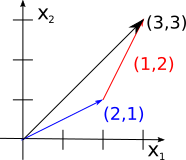
\includegraphics[scale = .30]{1.png}
\end{figure}

As you can see, the graph of this equation is a \textbf{straight line}, which is true for all linear equations



\end{document}